\begin{figure}[!htbp]
\centering
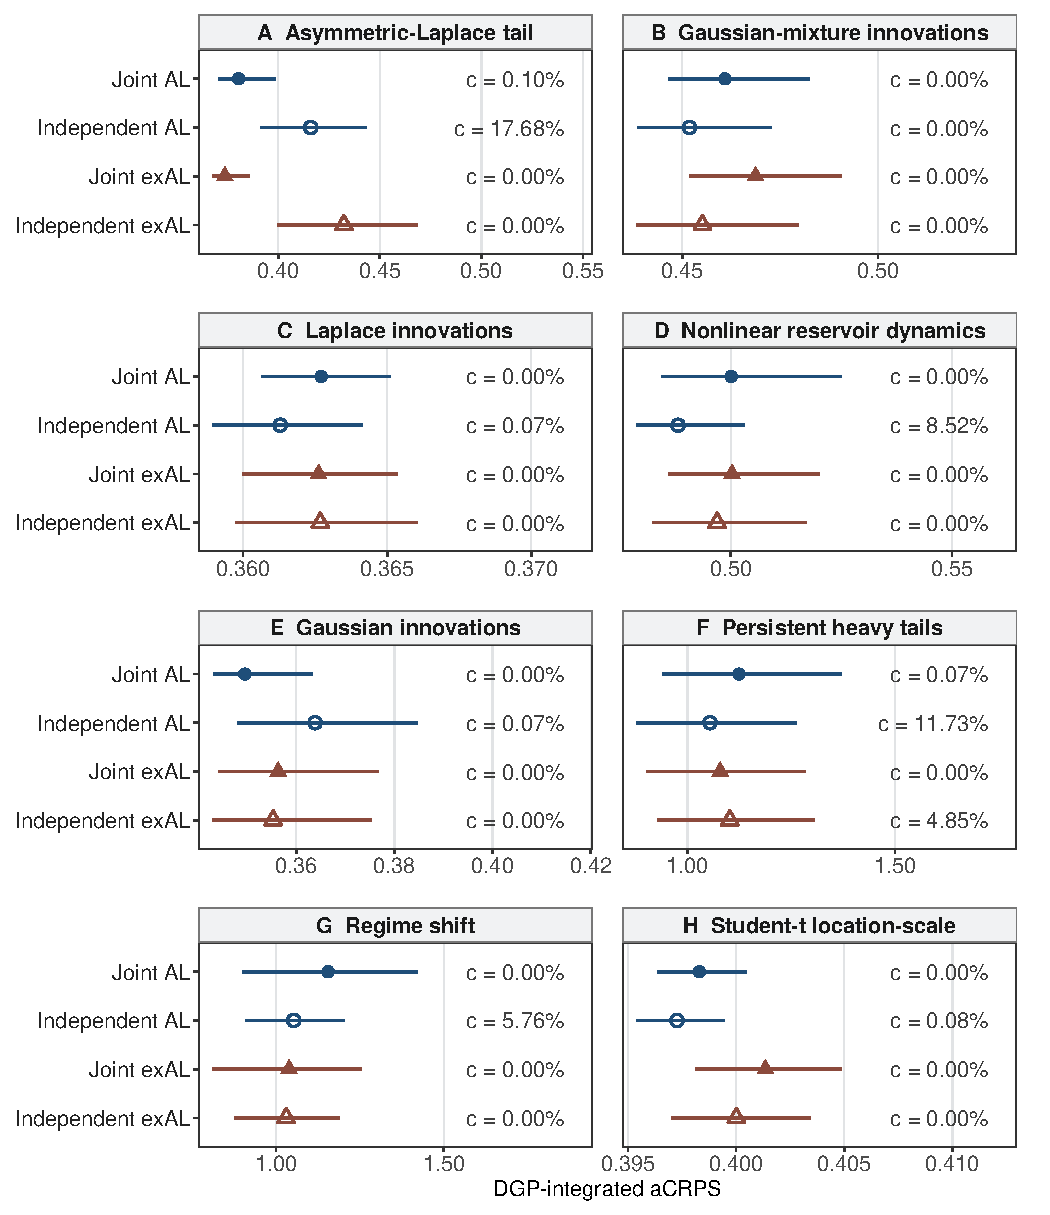
\includegraphics[width=0.94\textwidth]{figures/joint_qdesn_simulation/joint_qdesn_pure_desn_v2_forecast_dgp_acrps.pdf}
\caption{DGP-integrated \(\aCRPS\) for the pure-DESN multi-quantile study. Points are posterior means and segments are equal-tailed 95\% intervals, conditional on each model's averaged recursively generated forecast design. Lower scores are better. The annotations \(c\) give raw adjacent-level crossing percentages for the posterior-mean grids; every grid is monotone after projection. All winner and runner-up marginal intervals overlap.}
\label{fig:joint-qdesn-pure-desn-v2-forecast-acrps}
\end{figure}
